\documentclass{article}

\usepackage[americanvoltages,siunitx]{circuitikz}

\usepackage{menukeys}

\usepackage{hyperref}


\usepackage{color,soul}
\definecolor{lightblue}{rgb}{.90,.95,1}
\sethlcolor{lightblue}

\usepackage{graphicx}
\graphicspath{ {./images/} }

\usepackage{fancyhdr}
\chead{Written by Neil Johari}

\usepackage{ifthen}

\makeatletter
  \def\pgf@circ@drawvoltagegenerator{
    \ifpgf@circuit@bipole@voltage@below
        coordinate (pgfcirc@Vcont1) at ($(\ctikzvalof{bipole/name}.center) ! \ctikzvalof{voltage/bump a} ! (\ctikzvalof{bipole/name}.-120)$)
        coordinate (pgfcirc@Vcont2) at ($(\ctikzvalof{bipole/name}.center) ! \ctikzvalof{voltage/bump a} ! (\ctikzvalof{bipole/name}.-60)$)
    \else
        coordinate (pgfcirc@Vcont1) at ($ (\ctikzvalof{bipole/name}.center) ! \ctikzvalof{voltage/bump a} ! (\ctikzvalof{bipole/name}.120)$)
        coordinate (pgfcirc@Vcont2) at ($ (\ctikzvalof{bipole/name}.center) ! \ctikzvalof{voltage/bump a} ! (\ctikzvalof{bipole/name}.60)$)
    \fi

    \ifpgf@circuit@europeanvoltage
        \ifpgf@circuit@bipole@voltage@backward
            (pgfcirc@Vcont2)  -- node[currarrow, sloped,  allow upside down, pos=1] {} (pgfcirc@Vcont1)
        \else
            (pgfcirc@Vcont1)  -- node[currarrow, sloped,  allow upside down, pos=1] {} (pgfcirc@Vcont2)
        \fi

    \else % american voltage

        \pgfextra{
            \edef\pgf@temp{\pgfkeysvalueof{/tikz/circuitikz/bipole/kind}}
            \def\pgf@circ@temp{battery}
            \ifx\pgf@temp\pgf@circ@temp
                \def\pgf@circ@batteria{battery}
            \else
                \edef\pgf@circ@temp{battery1}
                \ifx\pgf@temp\pgf@circ@temp
                    \edef\pgf@circ@batteria{battery}
                \else
                    \edef\pgf@circ@batteria{false}
                \fi
            \fi
            \def\pgf@circ@temp{battery1}
        }

        \ifx\pgf@temp\pgf@circ@temp % if it is a battery, must put + and -
            \ifpgf@circuit@bipole@voltage@backward
                (pgfcirc@Vcont2)  node[xshift=2pt,yshift=-6pt] {$-$}  (pgfcirc@Vcont1) node[xshift=-2pt,yshift=-6pt] {$+$}
            \else
                (pgfcirc@Vcont1)  node[xshift=-2pt,yshift=-6pt] {$-$}  (pgfcirc@Vcont2) node[xshift=2pt,yshift=-6pt] {$+$}
            \fi
        \fi

    \fi
}
\makeatother

\title{Extra Lab: LTSpice Lab 2}
\date{Winter 2020}
\author{Engineering 100-950}

\begin{document}

\maketitle

\thispagestyle{fancy}

\section*{Learning Objectives}

\begin{itemize}
  \item You will be able to construct basic circuits using LTSpice software
  \item You will be able to analyze the result of LTSpice of simulations
\end{itemize}

\section*{Learning Assessments}

\begin{itemize}
  \item How does the SPICE engine programmatically analyze circuits?
  \item What is a ballast resistor?
  \item What SPICE directive do we use to perform a DC operating point simulation?
  \item Simulate a basic battery, lamp, and resistor in series using LTSpice, and retrieve the operating point analysis results.
  \item Why is SPICE useful in analyzing circuits with elements like diodes?
\end{itemize}

\section*{Lab Assignment}

Estimated completion time: ~0.5 hours +- 30 minutes. The variation depends heavily on skill level coming in, and the majority of time is expected to be reading the material in this lab and grasping concepts.

Please contact an IA if you are having difficulties and are spending more time than this!

I care more about you trying the problems and providing deliverables (the LTSpice screenshots proving you played with the software) than the fact that your answers are correct. This is a lot of work and you're not expected to do everything correctly!!

\begin{itemize}
  \item You will simulate two circuits: a basic circuit with only devices which follow Ohm's law, and another circuit with a non-linear device. You will then analyze this circuit and discuss the results. (30-60 minutes).
  \item You will Slack message either Neil or Sarah (will be a chat which may involve answering some basic conceptual questions, and going over your submission).
\end{itemize}

\section{Introduction}
The goal of this lab is to allow you to explore these concepts further to expose you to some of the basics of Electrical Engineering.

In lab 1, we covered some concepts surrounding basic circuit analysis. In this lab, you will use LTSpice to simulate circuits.

Many of the concepts we cover here are a preview of what you might learn in a course like EECS 215. If you enjoy this lab and the concepts of it, please consider taking the course!

If you find these concepts easy, consider completing the advanced version of this lab written by Sarah. In that lab, you get to explore basic first order circuits.

\subsection{Credits}
All tables and examples are from the EECS 215 course and book. Much of the wording is almost verbatim from the book, though topics were hand picked and distilled to prepare you for this lab. In particular, the course uses `Circuit Analysis and Design' by Fawwaz T Ulaby, Michael M. Maharbiz, and Cynthia M. Furse.

The assignments are taken directly from Lab 1 of the course, which means that if you choose to take the course, you're already (very slightly) ahead! After this lab you'll have played with LTSpice, which most students entering the course haven't... this will make all the labs significantly easier to work with.

This book can be freely downloaded here. It is not required to complete this lab or understand all the material, but may serve as a helpful reference if you need a more detailed primer than we provide here.

\subsection{Pre-requisites}
I assume you are familiar with the concepts of charge, current, and voltage. If
you are not, please read the `Circuits Primer' on Canvas under \menu{Files >
Labs > Introductory Documents > Circuits\_Primer.pdf}. 

This is an excellent way to intuitively grasp voltage and how it relates to current.

Additionally, I assume you're familiar with basic circuit analysis. Refer to lab one if you aren't familiar with circuit basics and nodal analysis.

\section{SPICE from LTSpice}
SPICE is an analog electronic circuit simulator that can help predict circuit behavior by fully simulating it. The guts of SPICE utilize nodal analysis to programmatically calculate all node voltages—this is why we had you learn and apply nodal analysis. SPICE is extremely old software and we do not interface with it directly.

LTSpice is freeware that implements the SPICE engine, and is the most popular software for interfacing with SPICE. The software includes a graphical interface that can be used with Windows and Mac OS X, and is available on CAEN computers.

LTspice is available at the link below, which also includes documentation on a
‘Getting Started Guide’ and shortcuts for Mac OS X:
\url{http://www.linear.com/designtools/software/#LTspice}

Please note that the Windows and Mac interfaces are very different. If you are on Mac, it will be harder and you can make it easier for yourself by having the Mac OS X shortcuts page open while you work.

\section{Creating Your Circuit}

You should begin by creating a new schematic (\menu{New > Schematic}). Then you add your components and wire them together.

\begin{itemize}
  \item Add new components. Use the \hl{voltage} and \hl{res} components for this lab.
    \begin{itemize}
      \item Windows: \menu{Edit > Component}
      \item Mac: \menu{Draft > Component}
    \end{itemize}
  \item Add a reference ground node
    \begin{itemize}
      \item Windows: Press ground from the menu bar.
      \item Mac: \menu{Draft > Net Name}, select GND (global node 0) and place.
    \end{itemize}
  \item Connect components with wires.
    \begin{itemize}
      \item Windows: \menu{Edit > Draw} Wire
      \item Mac: \menu{Draft > Wires}
    \end{itemize}
  \item Define component values by right clicking on each component and changing
    the value.

\end{itemize}

\section{Running a Simulation}

LTSpice can perform lots of different kinds of simulations, specified by a `SPICE Directive'. The simulation mode you will use in this lab is called the `DC operating point'.

Windows: \menu{Simulate > Edit} Simulation Command. Then choose \hl{DC op pnt}, click OK, and place the text anywhere on the schematic.

Mac: \menu{Draft > SPICE} Directive, type \hl{.op}, and place the text anywhere in the schematic.

Now press \hl{Run} (the running person icon).

\section{LTSpice Assignment 1}

\begin{figure}[h]
\centering
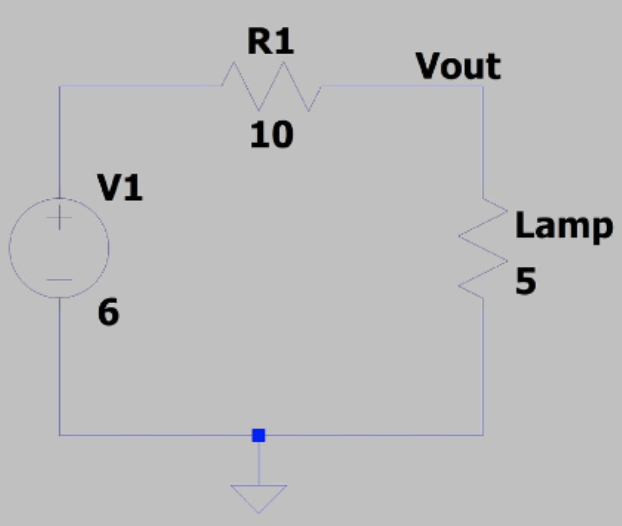
\includegraphics[width=0.5\textwidth]{lab1_fig-2}
\caption{Basic lamp circuit}
\label{fig:assignment1}
\end{figure}

Simulate the circuit Figure \ref{fig:assignment1}, and obtain the two
screenshots from Figure \ref{fig:assignment1_results}.

\begin{figure}[h]
\centering
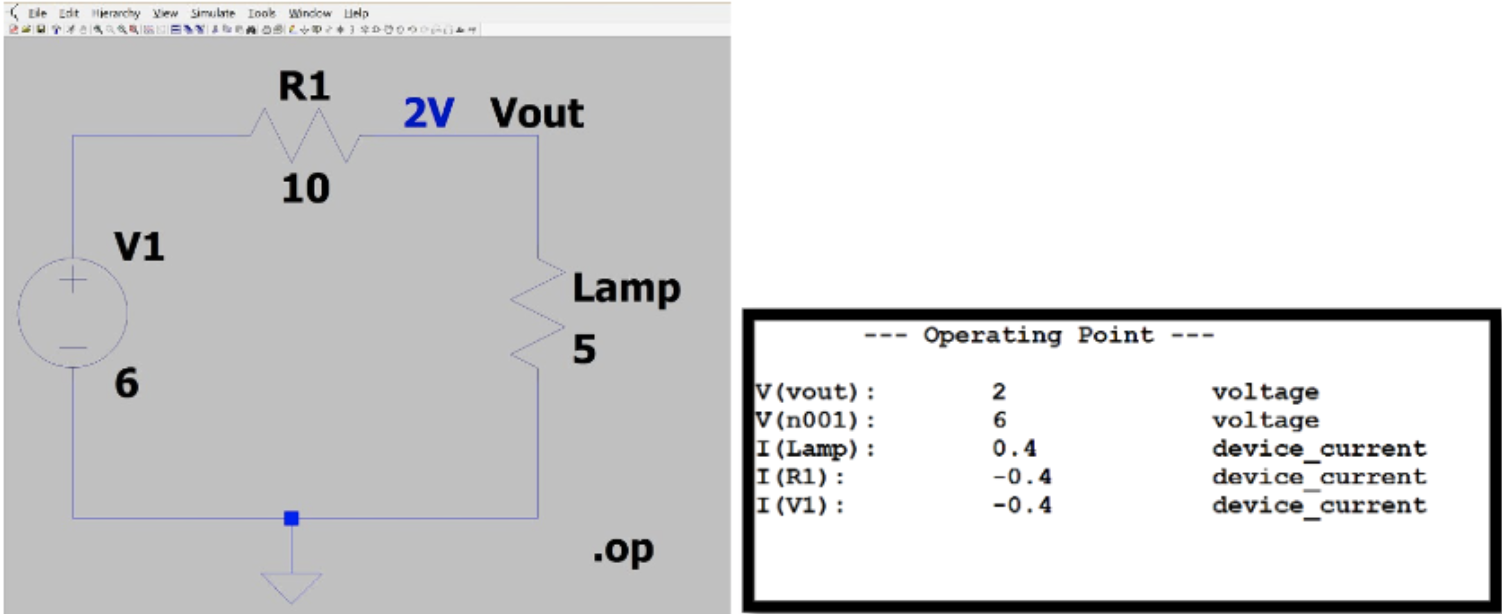
\includegraphics[width=0.65\textwidth]{lab1_fig-3}
\caption{Lamp circuit simulation results}
\label{fig:assignment1_results}
\end{figure}

\section*{LTSpice Assignment 2}

From our DC op point simulation, we see that 0.4 A pass through our lamp. Let's suppose that the manufacturer recommends we should only give 0.3 A max to our lamp, otherwise it will explode...

In order to make our circuit safe while still operating at 6V, we should play with our resistor's resistance to impede current until we are at 0.3 A. A resistor used to reduce current or voltage in a circuit is called a ballast resistor.

SPICE is a powerful tool that can help us do this pragmatically by sweeping different resistor values. To do this, perform the following steps:

\begin{itemize}
  \item Change the resistance value to the text \hl{\{ballast\}} (this makes the resistance a variable called ballast).
  \item Define a new SPICE directive \hl{.step param ballast 5 20 0.5}. This will sweep through different values for ballast.
    \begin{itemize}
      \item The format for this command is \hl{.step param variable start end stepsize}.
    \end{itemize}
  \item Run the simulation and in your waveform window add a trace for \hl{I(Lamp)}. This will give you \hl{I(Lamp)} vs \hl{R1}.
\end{itemize}

Take a screenshot of your modified circuit and the waveform window you obtained for submission. Additionally, submit your answer to this question: What resistance value limits the current to .3 Amps? (Hint: You can double check your answer with Ohm's law, since our lamp is a linear resistor!).

\section*{LTSpice Assignment 3}
The lamp circuit is something we could've done by hand with almost no issue. This is because the lamp had a linear i-v characteristic (it obeyed Ohm's law). Not all devices are ohmic, however...

The most accessible example of a non-linear device that you have already in fact used in previous labs is the LED. LED stands for `light emitting diode', and diodes are typically non-linear devices.

Figure \ref{fig:assignment3} is an example of one such non-linear circuit.

\begin{figure}[h]
\centering
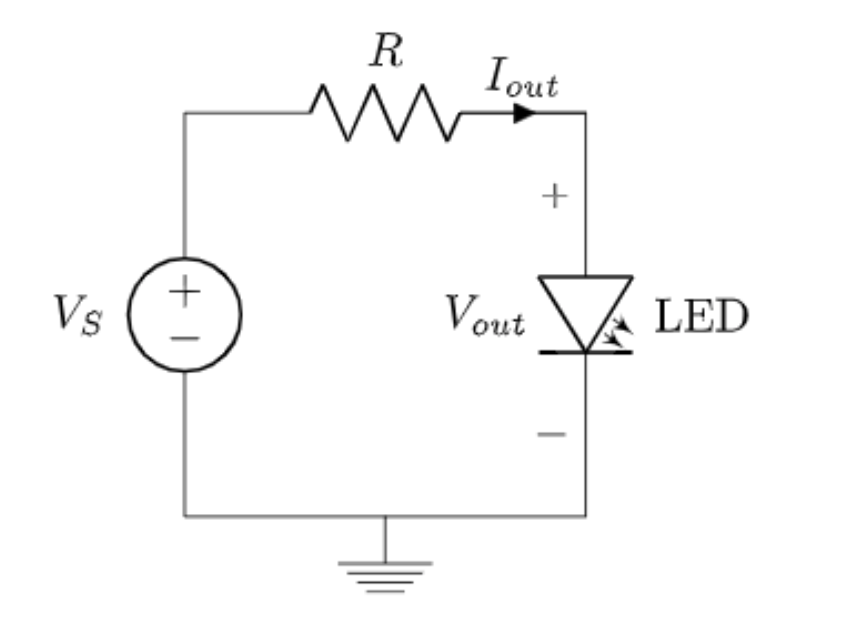
\includegraphics[width=0.65\textwidth]{lab1_fig-15}
\caption{LED circuit diagram}
\label{fig:assignment3}
\end{figure}

\begin{itemize}
  \item For this assignment, draw the circuit above using the LED component.
    There are many LEDs, but for this task right-click the LED and choose
    \menu{Pick New Diode > LXHL-BW02} 
  \item Define the resistance value R as 0.1 Ohms.
  \item Similar to how we sweeped in the lamp circuit, use a SPICE directive
    \hl{.dc v1 0 4 0.01} to sweep the voltage source v1 from 0V to 4V in steps of 0.01V.
  \item Plot the I(Led) in the waveform window, and change the scale of the current axis to values between 0-0.5A.
\end{itemize}



\section*{What to submit for this lab}

\begin{enumerate}
  \item Your solution to `LTSpice Assignment 1'
    \begin{itemize}
      Include both screenshots (the schematic and operating point results)
    \end{itemize}
  \item Your solution to `LTSpice Assignment 2'
    \begin{itemize}
      \item Include both screenshots (the modified schematic and waveform
        window)
      \item Include your answer to the question `What resistance value limits
        the current to 0.3 Amps'

    \end{itemize}
  \item Your solution to `LTSpice Assignment 3'
    \begin{itemize}
      \item Include the screenshot of your waveform window
    \end{itemize}
  \item Don't forget to Slack message either Neil or Sarah!
\end{enumerate}

 \end{document}
